My goal of pairing bugs with social media might be somewhat similar to nowadays very active field of bug report duplicate discovery but has also a lot common with topic modeling and general text similarity algorithms.

To link any two texts based on their content, there's an obvious need for understanding what the text features are. 
To do this, there are several ways how to calculate text (string) similarity value or one can even execute so called "Topic modeling" algorithm and try to connect documents based on their matching topics.

Topic modeling is a method used to organize and summarize large textual information. It's used to discover hidden topical patterns and annotate documents according to these topics. It can also be described as a method of finding group of words (i.e topic) from in a text that best represents the information in the collection.

The obstacle of using a topic modeling for my case is that output is not granular enough to differentiate among similar texts which are all from the very same domain. Because the output provided by topic modeling wasn't enough to pair particular items, I searched for, found and considered several alternative approaches.

\section{Aproaches}
There are many ways and approaches how to find out whether 2 texts share some common topic. Most of them are to some extent very similar as the general rule is to extract textual features and compare them using statistical approaches. Common way to do this is to transform documents into vectors and then compute cosine similarity between them. These text transformations are implemented in several Python packages.\\
\\
I have tried following:
\begin{enumerate}
\item String similarity using NLTK
\item String similarity using Scikit-learn
\end{enumerate}

\paragraph{NLTK:}First step in calculating similarity was to tokenize the text. NLTK offers several types of tokenizers with various outputs. Text tokenization can operate on various levels and the structure of input has to be considered. As I am comparing the whole documents and do not want to consider sentences as standalone objects, I have chosen to use \textit{nltk.tokenize.wordtokenize} method instead of e.g. \textit{nltk.tokenize.senttokenize}.\\
Next step after the document is tokenized is to stem the words. Stemmers remove morphological affixes from words, leaving only the word stem. Once again as with tokenizers, there are several stemmers implemented within NLTK. After doing a short research I have come to conclusion that as far as I use the same stemmer for both, Git issues and SO/Reddit entries, it should not play any major role in results.\\
Next step is getting rid of stop words. These usually refer to the most common words in a language, but there is no single universal list of stop words used by all natural language processing tools. The set of stop words defined for my NLTK version had a size of 153.\\
Listing \ref{lst:nltkTextSimilarity} illustrates the implementation of the described similarity calculation procedure.

\begin{lstlisting}[caption={Text similarity implementation with NLTK},label={lst:nltkTextSimilarity},language=Python]
		tokens = word_tokenize(text)
		words = [w.lower() for w in tokens]

		porter = nltk.PorterStemmer()
		stemmed_tokens = [porter.stem(t) for t in words]

		# removing stop words
		stop_words = set(stopwords.words('english'))
		filtered_tokens = [w for w in stemmed_tokens if not w in stop_words]

		# count words
		count = nltk.defaultdict(int)
		for word in filtered_tokens:
			count[word] += 1
		return count;
\end{lstlisting}

After the previous 3 steps are executed on both documents, 2 vectors from all words from both documents are created. Each documents then sets the counts of words it contains and a cosine similarity of these two "count vectors" is calculated. This similarity calculation is a basic similarity calculation and could definitely be optimized. For example, it does not analyse and consider role and position of word in a sentence (POS tagger would be required here). 

\paragraph{Scikit-learn and TF-IDF:}There are several ways to assess the importance of each feature by attaching a certain weight in the text. The most
popular ones are: feature frequency (FF), Term Frequency Inverse Document Frequency (TF-IDF), and feature presence
(FP) \cite{haddi2013role}. My next similarity checker I have implemented was using Scikit-learn module and TF-IDF vectorizer. While BoG only takes into consideration the frequency of words in a document TF-IDF reflects how important a word is for the particular document. For a word to have high TF-IDF in a document, it must appear a lot of times in said document and must be absent in the other documents. It must be a signature word of the document.\\
\\
Term frequency represents how often is the word present in the said document. Simplest approach is the raw count.
\[ tf_{count}(t,d) = f(t,d) \]
Other options include term frequency adjusted for document length, logarithmically scaled frequency or augmented frequency to handle bias towards longer documents.\\
Inverse document frequency is a counterweight factor which diminished importance of terms that appear in the set very often in the document set and therefore increases the weight of terms that occur rarely.
\[ idf(t) = log \frac{N}{df(t)} \]
The final weighing scheme combines term frequency and inverse document frequency.
\[ tfidf(t,d) = tf(td) x idf(t)		\]
Listing \ref{lst:scikitkTextSimilarity} shows my very simple implementation of TF-IDF similarity checker using Scikit-learn module.

\begin{lstlisting}[caption={Text similarity implementation with Scikit using Tf-Idf model},label={lst:scikitkTextSimilarity},language=Python]
		def getSimilarity(self,text1, text2):
			tfidf = self.vect.fit-transform([text1, text2])
			return (tfidf * tfidf.T).A
\end{lstlisting}

\paragraph{Stack Overflow questions preprocessing:}  Online texts contain usually lots of noise and uninformative parts such as HTML tags, scripts and advertisements \cite{haddi2013role}. Before running implemented similarity algorithms, I have decided to preprocess the stack questions and get rid of code snippets within \textit{\textless pre\textgreater\textless code\textgreater} tags and hypertext links. Especially snippets could potentially effect (increase) the similarity score if kept in the text.

	

\section{Available data}
\paragraph{Git issue reports:}
Using the approach described in the section \ref{ssec:issuesMining}, I've downloaded 96,651 issue reports from Git while 25,978 of those labeled as bug or similar. Because this part of the thesis was more just a PoC than the part with sentiment analysis, I've decided not to work with all the data and rather just picked several projects of interest. The bug counts among this projects is displayed in the table \ref{table:projectIssuesDistribution}.


\begin{table}[H]
\centering
\begin{tabular}{ |p{3cm}||p{3cm}|}
 \hline
\textbf{ Framework }& \textbf{Bug count}\\
 \hline
 NodeJS   & 1615\\ \hline
 AngularJS &   2225 \\ \hline
 EmberJS & 1284\\ \hline
 VueJS & 353\\ \hline
 Aurelia & 73\\ \hline
 Bower & 155\\ \hline
\end{tabular}
\caption{Bug count per project}
\label{table:projectIssuesDistribution}
\end{table}

\paragraph{Stack overflow questions:}
SO mining has been described in section \ref{ssec:GettingData} and I've downloaded 5,847 questions. There are thousand questions for AngularJS, NodeJS, Bower, Ruby on Rails and VueJS each and EmberJS has only 847 questions. Downside is, that despite having a lot of questions, it doesn't necessarily mean that each and every one of them talks about some known bug. Actually, opposite is true as out of all those questions only very tiny percentage does (AngularJS - 1, NodeJS - 2, EmberJS - 2, VueJS - 0).

\paragraph{Reddit dialogues:}Reddit subreddits mining has been described in the same subsection as SO mining. Results of this process are shown in the table \ref{table:redditDiscussionsDistribution}.


\begin{table}[H]
\centering
\begin{tabular}{ |p{3cm}||p{3cm}|}
 \hline
\textbf{ Framework }& \textbf{Submissions count}\\
 \hline
 NodeJS   &  108\\ \hline
 AngularJS &   43 \\ \hline
 VueJS & 20\\ \hline
 EmberJS & 13\\ \hline
\end{tabular}
\caption{Reddit submissions counts}
\label{table:redditDiscussionsDistribution}
\end{table}


\section{Similarity results}
Linking items and in general finding similarity among these already area-specific texts proved to be a problematic task. To test my algorithm I decided to compare 89 SO questions with its matching Git issue and 4x one random git issue of the project. Results are plotted in Figure \ref{fig:MatchesVsRandom}.\\

\begin{figure}[H]%
    \centering
	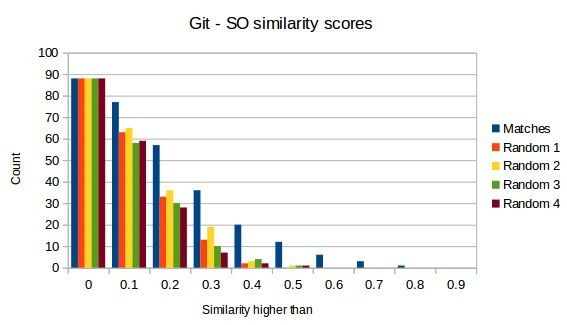
\includegraphics[width=15cm]{MatchesVsRandom.jpg}
    \caption{Similarity distribution of 89 matches and four data series of 89 random pairs}%
    \label{fig:MatchesVsRandom}%
\end{figure}
Results very clearly show that there is a particular similarity score, which is very hard to pass for two unrelated items. This score is obviously not constant and it depends on implementation of the similarity calculation. For my NLTK BoW algorithm used in Figure \ref{fig:MatchesVsRandom}, the threshold is 0.4 or 0.5. Choosing the value of threshold would also depend on the  desired characteristics of a classifier and the prioritized metric. For example if a precision would be more important than recall, the ideal threshold would be 0.7 as it is the value which has never been passed by any of 356 non-matching pairs. The detailed table with the values for a Figure \ref{fig:MatchesVsRandom} can be seen in appendix.\\
\\
I have executed the same steps using the TF-IDF approach and although the values are different (as expected), they follow the same pattern. Figure \ref{fig:MatchesVsRandom_TfIdf} demonstrates these results and detailed values can again be found in appendix.

\begin{figure}[H]%
    \centering
	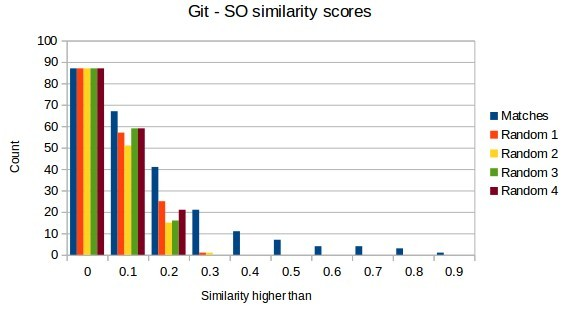
\includegraphics[width=15cm]{MatchesVsRandom_TfIdf.jpg}
    \caption{Similarity distribution of 89 matches and four data series of 89 random pairs}%
    \label{fig:MatchesVsRandom_TfIdf}%
\end{figure}

Despite clearly seeing possible threshold values, an algorithm which would label all the pairs above this threshold as matches would achieve very bad recall around 30\%. On the other side, precision would be 100\%. The potential problem is that the real-world ratio between matching and non-matching pairs rises exponentially with every new item on any side (Git issue, SO question). Testing the algorithm on bigger amount of data in the future could answer the question whether the threshold around 0.3 really proves as a unbreakable resistance for unrelated Git-SO pairs.\\
\\
Although I was not successful to such extent that the output are Git-StackOverflow or Git-Reddit True Positive pairs, I have pointed out some interesting results and data relationships.

\label{ssec:similarityResultsSO}
\subsection{Stack Overflow}
The average similarity (using NLTK approach) between SO questions talking about particular issue and that particular issue description is 0.316 without body preprocessing and 0.292 with body preprocessing. The distribution of similarities in buckets by increased by 0.05 can be seen in histogram in Figure \ref{fig:GitStackMatchesHistogram}

\begin{figure}[H]%
    \centering
	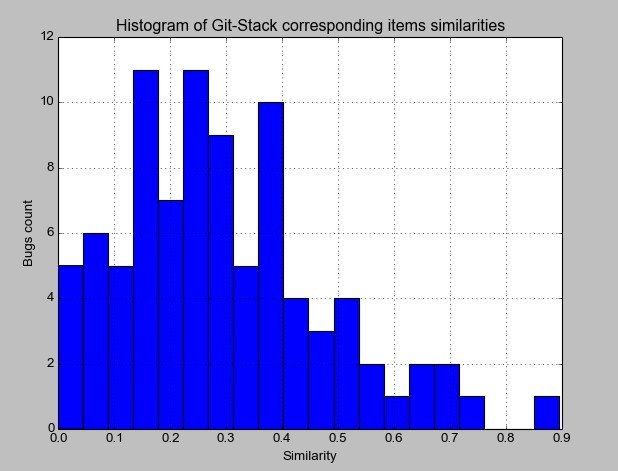
\includegraphics[width=8cm]{gitStackMatchesHistogram.jpg}
    \caption{Histogram of similarities distribution among git issues and their matching SO questions}%
    \label{fig:GitStackMatchesHistogram}%
\end{figure}

For random SO questions, amount of comparisons to Git issues needed to be limited. If every SO question would be compared to every Git issue, time of computation would exceed timeframe of this thesis. Every SO question was therefore compared to 20 random Git issues and resulting average similarity scores are in following figures.

\begin{figure}[H]%
    \centering
	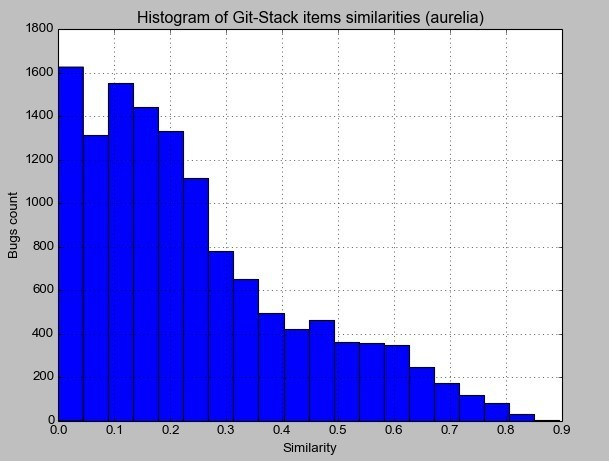
\includegraphics[width=8cm]{AureliaStackWithRandom20Bugs.jpg}
    \caption{Histogram of Aurelia SO questions and random git issues. Average similarity was 0.244}%
    \label{fig:AureliaStackWithRandom3Bugs}%
\end{figure}

\begin{figure}[H]%
    \centering
    \subfloat[EmberJS average similarity - 0.247]{{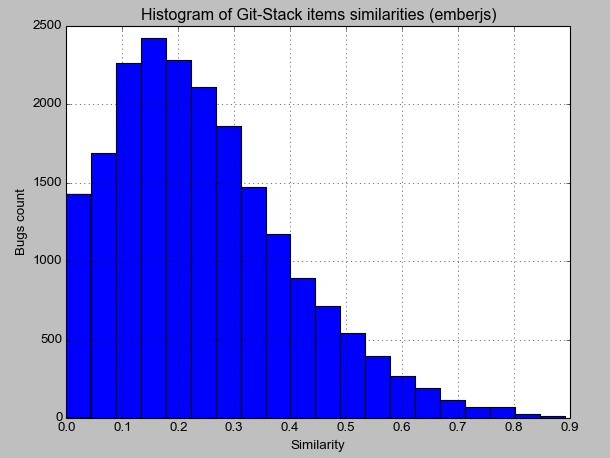
\includegraphics[width=5.5cm]{EmberStackWithRandom20Bugs.jpg} }}%
    \qquad
    \subfloat[Bower average similarity - 0.217]{{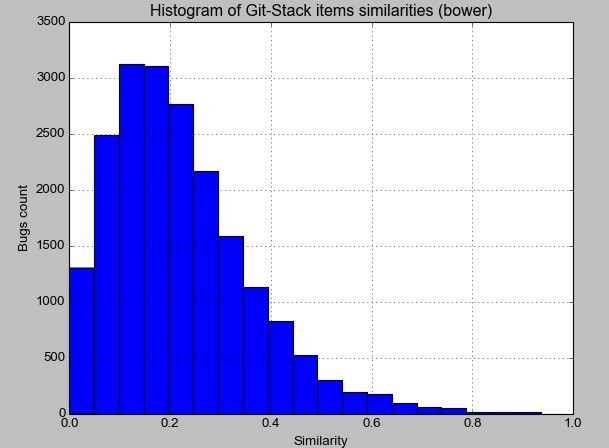
\includegraphics[width=5.5cm]{BowerStackWithRandom20Bugs.jpg} }}%
    \caption{EmberJS and Bower similarity histogram}%
    \label{fig:BowerEmberWithRandom3Bugs}%
\end{figure}

\begin{figure}[H]%
    \centering
    \subfloat[VueJS average similarity - 0.255]{{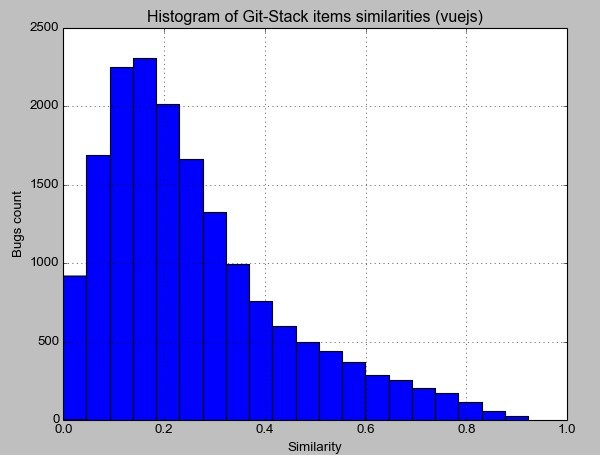
\includegraphics[width=5.5cm]{VueJSStackWithRandom20Bugs.jpg} }}%
    \qquad
    \subfloat[AngularJS average similarity - 0.258]{{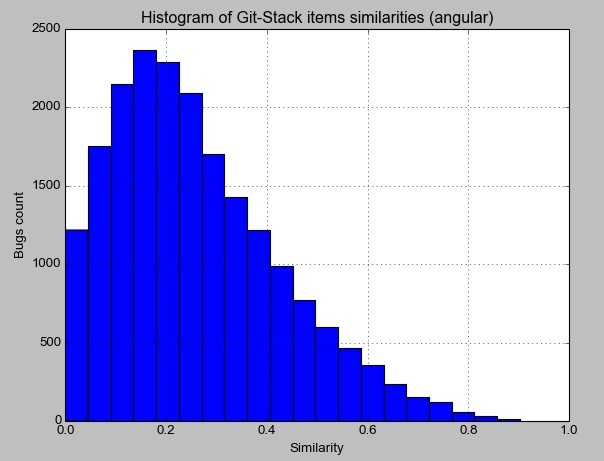
\includegraphics[width=5.5cm]{AngularStackWithRandom20Bugs.jpg} }}%
    \caption{VueJS and AngularJS similarity histogram}%
    \label{fig:VueAngularWithRandom3Bugs}%
\end{figure}


Table \ref{table:StackOverflowNLTKsimilarity} illustrates results of comparing Git bugs descriptions with SO questions talking about the same project issues and general issues. From values displayed, it is apparent that the difference between matches and random pairs is not very big. This is probably because all the texts about a particular project are already very specific and similar in their nature anyway.

\begin{table}[H]
\centering
\begin{tabular}{ |p{3cm}||p{4.5cm}|p{5.5cm}|}
 \hline
\textbf{ Framework }& \textbf{Own issues similarity}& \textbf{20 random issues similarity}\\
 \hline
 NodeJS   & 0.265 & 0.243\\ \hline
 AngularJS & 0.241 & 0.260\\ \hline
 EmberJS & 0.282 & 0.246\\ \hline 
 VueJS &   0.261 & 0.258\\ \hline
\end{tabular}
\caption{NLTK similarity values for SO questions}
\label{table:StackOverflowNLTKsimilarity}
\end{table}

\subsection{Reddit}Here I have calculated the similarity between the bug description and either particular comment in the Reddit discussion which mentioned the bug or the whole discussion itself. Using NLTK BoW approach, average similarity score for all considered projects (NodeJS, AngularJS, VueJS and EmberJS) was 0.481 for the whole discussion and 0.368 for the comment itself. Scikit If-Idf values were 0.263 and 0.207 respectively. Detailed scores for each project can be found in Table \ref{table:RedditNLTKsimilarity} for NLTK implementation and Table \ref{table:RedditSCIKITsimilarity} for Sci-kit. Subreddit for EmberJS did not reference any of its own bugs.

\begin{table}[H]
\centering
\begin{tabular}{ |p{3cm}||p{3cm}|p{4cm}|}
 \hline
\textbf{ Framework }& \textbf{Bug comment}& \textbf{Whole discussion}\\
 \hline
 NodeJS   & 0.447 & 0.507\\ \hline 
 AngularJS & 0.306 & 0.57 \\ \hline 
 VueJS &   0.359 & 0.380\\ \hline
\end{tabular}
\caption{Reddit NLTK similarity values}
\label{table:RedditNLTKsimilarity}
\end{table}

\begin{table}[H]
\centering
\begin{tabular}{ |p{3cm}||p{3cm}|p{4cm}|}
 \hline
\textbf{ Framework }& \textbf{Bug comment}& \textbf{Whole discussion}\\
 \hline
 NodeJS   & 0.255 & 0.328\\ \hline 
 AngularJS & 0.168 & 0.278 \\ \hline 
 VueJS &  0.209  & 0.208\\ \hline
\end{tabular}
\caption{Reddit Scikit similarity values}
\label{table:RedditSCIKITsimilarity}
\end{table}

Both similarity calculations indicate that the semantic meaning of the bug is better expressed in the whole discussion rather than just the particular comment which referenced the bug. This made me question if it could be generalized that longer the text is, more similar it is to actual bug description. I have plotted a relationship between similarity score and length for Reddit in Figure \ref{fig:SimilarityLengthRelationshipComment} and the same for Stack Overflow discussion can be seen in Figure \ref{fig:GitStackSimilarityWeightedScatter}.

\begin{figure}[H]%
    \centering
    \subfloat[Discussion lengths]{{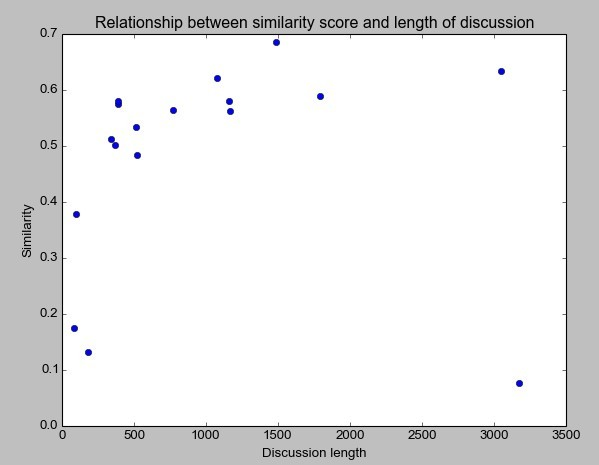
\includegraphics[width=5.5cm]{SimilarityLengthRelationshipDiscussion.jpg} }}%
    \qquad
    \subfloat[Comment lengths]{{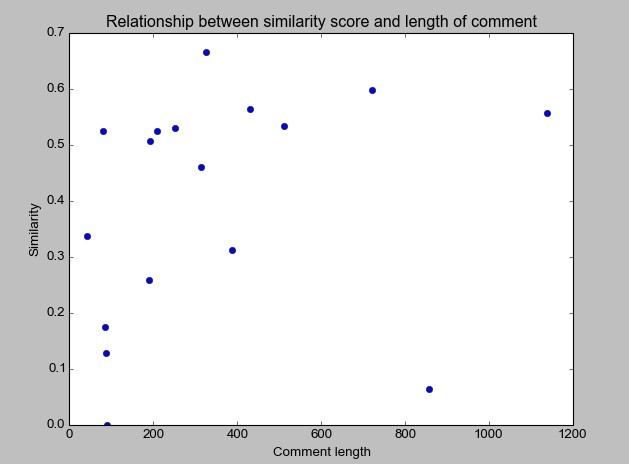
\includegraphics[width=5.5cm]{SimilarityLengthRelationshipComment.jpg} }}%
    \caption{Text lengths and similarity scores with matching issues}%
    \label{fig:SimilarityLengthRelationshipComment}%
\end{figure}

\begin{figure}[H]%
    \centering
	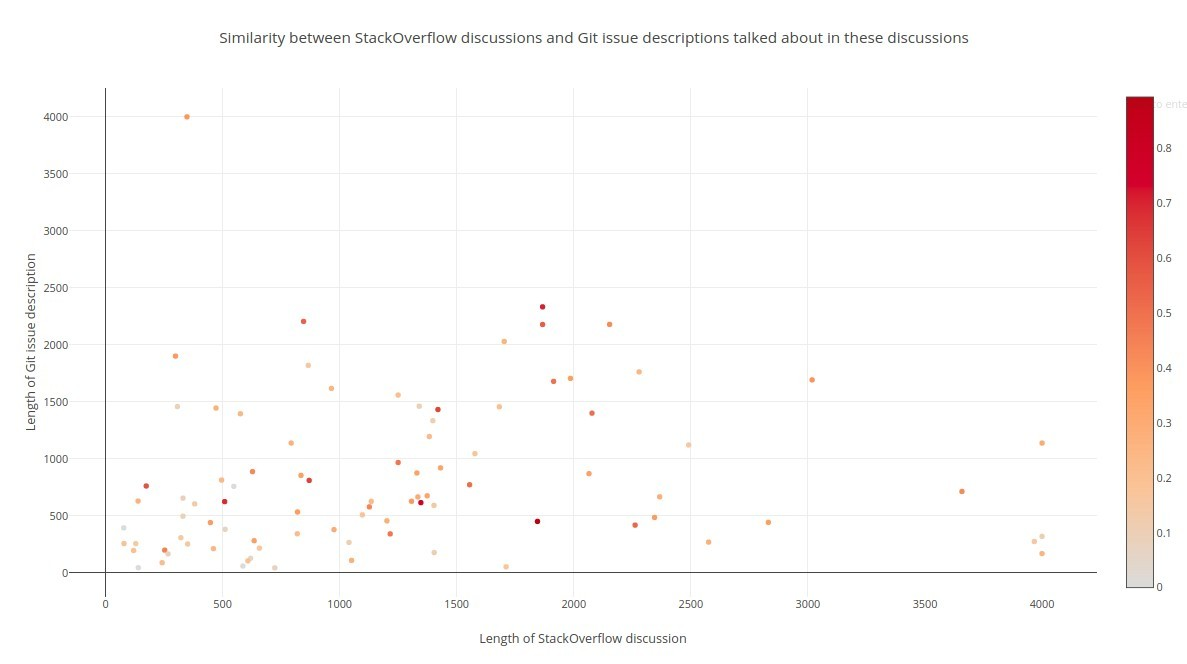
\includegraphics[width=10cm]{GitStackSimilarityWeightedScatter.jpg}
    \caption{Git and SO discussion lengths and similarity scores with the issue}%
    \label{fig:GitStackSimilarityWeightedScatter}%
\end{figure}


\section{Using GIT labels}
One more considered approach how to recognize an issue's topic was using the GIT labels. Labels on GitHub help you organize and prioritize your work. You can apply labels to issues and pull requests to signify priority, category, or any other information you find useful. There are two types of labels - default and custom. GitHub provides default ones in every new repository. All default labels can be seen in table \ref{fig:defaultLabels} and can be used to create a standard workflow in a repository:

\begin{figure}[H]%
    \centering
	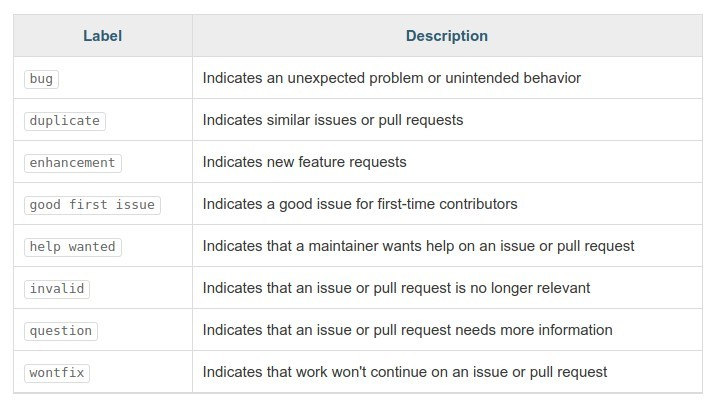
\includegraphics[width=8cm]{defaultLabels.jpg}
    \caption{Default Git labels provided for every repository}%
    \label{fig:defaultLabels}%
\end{figure}

These default labels come as a big help in directing the project and targeting the most important issues, but they don't say much about the nature of the issue itself.

The custom tags tell are used to specify the part of the project, where the issue is located but they still don't give any semantic information about the issue itself. That's the reason why this approach was rejected. 

